\chapter{Theoretische Grundlagen}
\section{Oberfl�chenplasmonen}
Ein \emph{Plasma} ist ein Gas aus freien Ladungstr�gern mit Gesamtladung 0 --
so zum Beispiel ein vollst�ndig ionisiertes Gas. Im Rahmen des Drude-Modells der
quasifreien Elektronen in einem metallischen Festk�rper kann man die bis auf
reibungsartige Kr�fte freien Leitungselektronen als Plasma betrachten.
In einem solchen Elektronenplasma als Medium k�nnen sich Ladungstr�gerdichteschwankungen
als Wellen fortpflanzen. Man nennt eine solche sich fortpflanzende Plasmawelle
\emph{Plasmon}.

In einem Volumen aus Plasma gilt f�r eine sich als ebene Welle
fortpflanzende Elektronendichteschwankung, dass das erzeugte elektrische Feld
stets parallel zum $k_{\text{VP}}$--Vektor ist, den man der ebenen Plasmawelle (dem
\emph{Volumenplasmon}) zuordnet. Da bei elektromagnetischen Wellen der entsprechende
$k$--Vektor immer senkrecht auf dem $E$-Feld steht, kann es daher �ber das elektrische
Feld keine Kopplung zwischen Licht und Volumenplasmonen geben.

Es gibt auch sogenannte \emph{Oberfl�chenplasmonen}, die Ladungsdichteschwankungen
in der Grenzfl�che zwischen einem Metall und einem Isolator entsprechen. Wie in
Abbildung \ref{fig:op} illustriert, f�hren diese nahe der Grenzfl�che auch zu dieser
senkrechte Anteile des elektrischen Felds mit sich.

\begin{figure}[ht]
    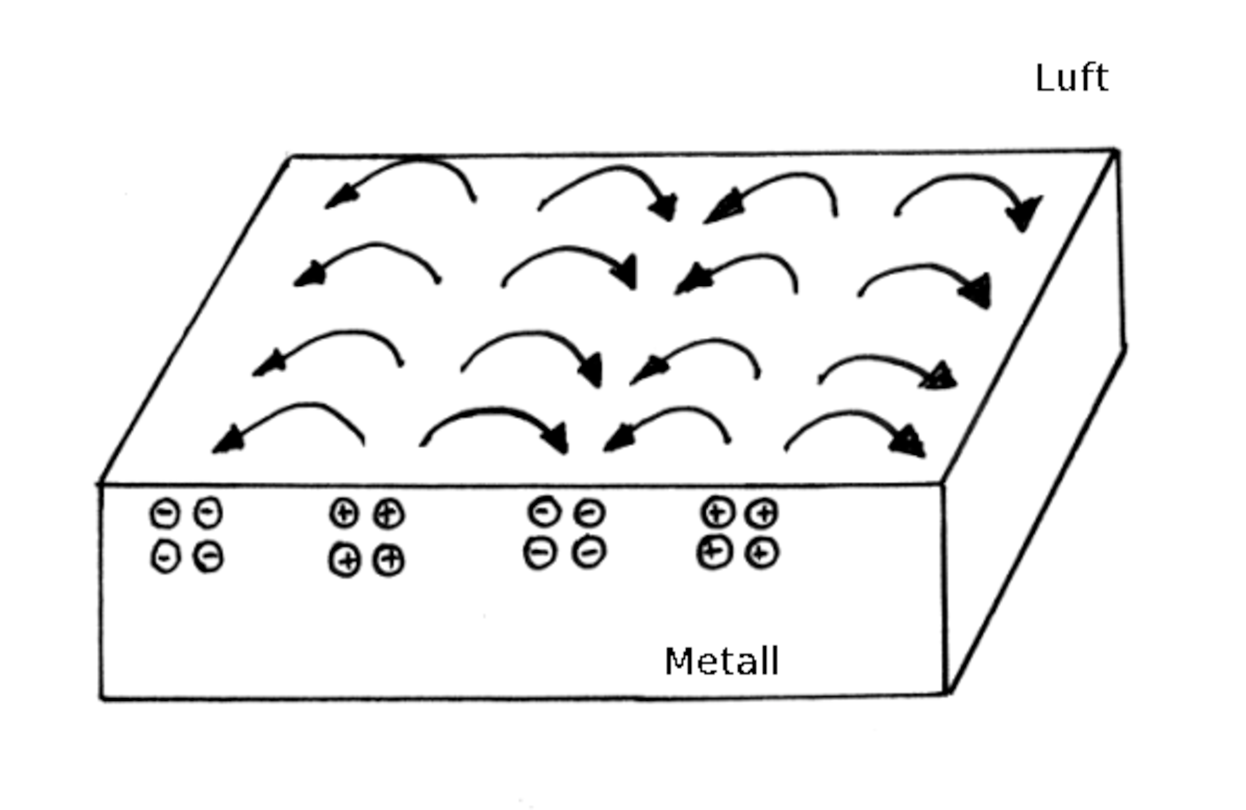
\includegraphics[width=0.8\textwidth]{op-.pdf}
	\caption{Oberfl�chenplasmonen in der Grenzschicht zwischen Metall und Luft}
	\label{fig:op}
\end{figure}

Es gibt dann potentiell Anregungen von Oberfl�chenplasmonen durch
bez�glich seiner Einfallsebene zur Grenzfl�che
$p$-polarisiertem Licht, mit einem $k_\text{OP}$--Vektor gleich der zur Grenzfl�che
parallelen Komponente des $k$--Vektors von Licht. Die Resonanzen dieser Anregung
geschehen bei �bereinstimmung von sowohl Frequenz $\omega$ als auch Wellenl�nge
$\frac{2\pi}{k}$ des zur Grenzfl�che
parallelen Anteils des Lichts und der Oberfl�chenplasmonen, also bei Schnittpunkten
der jeweiligen Dispersionrelationen zwischen $\omega$ und $k$.

\section{Dispersionsrelationen} \label{sec:disprel}

Die Dispersionsrelation von Oberfl�chenplasmonen in der Grenzschicht zwischen einem
Metall (2) mit Permittivit�t $\eps_2$ und einem Dielektrikum (1) mit Permittivit�t
$\eps_1$ ist
\begin{equation}	\label{eq:opdisp}
	k = \frac{\omega}{c}\sqrt{\frac{\eps_1\eps_2}{\eps_1+\eps_2}}
\end{equation}

Die Dispersionsrelation von Licht in einem Medium ($i$) mit Permittivit�t $\eps_i$
ist
\begin{equation}
	k = \frac{\omega}{c}\sqrt{\eps_i}
\end{equation}

Wenn Licht mit Einfallswinkel $\theta$ auf eine ebene Grenze des Mediums $(i)$ f�llt,
dann gilt damit f�r die
zur Ebene parallele Komponente $k_x$ des Licht--$k$--Vektors
\begin{equation}	\label{eq:lichtprojdisp}
	k = \frac{\omega}{c}\sqrt{\eps_i}\sin{\theta}
\end{equation}

\section{Permittivit�ten} \label{sec:perm}

Die Permittivit�t von Luft ist in guter N�herung 1.

F�r die Permittivit�t von Glas gibt es die empirische N�herungsformel

\begin{equation}
	\eps_\text{Glas}
	= 2,979864 + \frac{877780,8}{\frac{\lambda}{\mathring{A}}^2-1060900}
	- \frac{84,06224}{96-\frac{\lambda}{\mathring{A}}^2 10^{-8}}
\end{equation}

und f�r Silber haben wir

\begin{equation}
	\begin{split}
	\eps_\text{Ag}
	= &-219,945 - 0,0261695\frac{\lambda}{\mathring{A}}
	+ 3,8559 \sqrt{\frac{\lambda}{\mathring{A}}}
	+ \frac{4857,2}{\sqrt{\frac{\lambda}{\mathring{A}}}} \\
	&+ i(7,139 + 0,001656\frac{\lambda}{\mathring{A}}
	- 0,2129 \sqrt{\frac{\lambda}{\mathring{A}}})
	\end{split}
\end{equation}